\section{两类曲面积分的对比和意义}

本节首先对比两类曲面积分,分析它们的区别,再讨论它们的物理意义。

本节要点:
\begin{itemize}
    \item 理解“对曲面”和“对坐标平面”的含义;
    \item 理解曲面积分的物理意义。
\end{itemize}

%============================================================
\subsection{曲面积分的对比}

将三重积分和两类曲面积分放在一起,
\begin{align*}
&\iiint\limits_V{f\left( \boldsymbol{p} \right) dv} \\
&\iint\limits_S{f\left( \boldsymbol{p} \right) ds} \\
&\iint\limits_S{\boldsymbol{f}\left( \boldsymbol{p} \right) ^T\mathbf{n}\left( \boldsymbol{p} \right) \cdot ds}=\iint\limits_S{\boldsymbol{f}\left( \boldsymbol{p} \right) ^T\boldsymbol{ds}}
\end{align*}
可以看到:
\begin{itemize}
    \item 第一类曲面积分和三重积分的区别只在积分区域,前者是曲面,后者是三维体;
    \item 第一类曲面积分的积分区域是一个曲面,所以又称{\bf 对曲面面积的积分};
    \item 第二类曲面积分又可以写成坐标平面分量的形式,所以又称{\bf 对坐标平面的曲面积分};
    \item 两种曲面积分的区别在于被积函数,第二类曲面积分的被积函数是向量值函数在切面法方向上的投影$\boldsymbol{f}\left( \boldsymbol{p} \right) ^T\mathbf{n}\left( \boldsymbol{p} \right) $,或者说第二类曲面积分的积分表达式是两个向量函数的内积$\boldsymbol{f}\left( \boldsymbol{p} \right) ^T\boldsymbol{ds}$;
    \item 计算方法上,都是化成重积分求解。
\end{itemize}

\begin{tcolorbox}
从式子上看,只要看到$ds$的都是第一类曲面积分,有$dxdy,dydz,dzdx$单独出现的就是第二类曲面积分。
\end{tcolorbox}

%============================================================
\subsection{曲面积分的物理意义}

物理上,第一类曲面积分表示一数量场对曲面的总量,如弧面的质量、非均匀带电球面的电荷总量等。
第二类曲面积分是计算一矢量场对曲面的总通量的问题,如果是电场,则通量就是通过该曲面的电通量,如果是水流,则通量就是流过该曲面的水流量。

举例说明,三维空间中,一个固定方向的流速均匀流速场通过一个垂直平面的流量为$v\cdot S$。
如果平面和流速场方向不一致,则需要引入它们之间的夹角$v\cdot S\cdot \cos \theta $,可以理解为平面在流速场方向的投影,也可以理解为两个矢量的内积$\boldsymbol{v}^T\boldsymbol{S}$。

\begin{figure}[h]
\centering
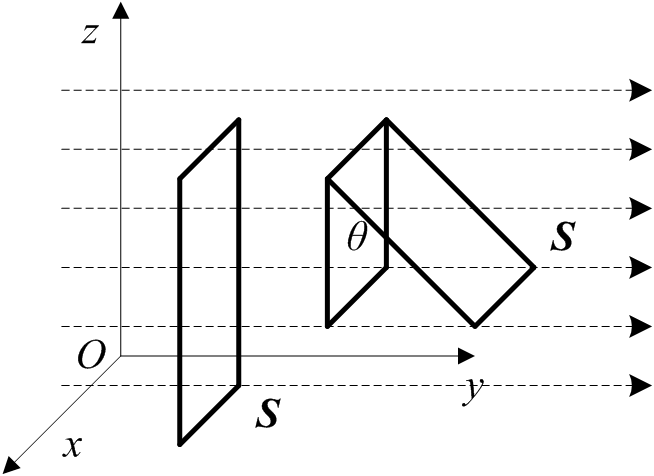
\includegraphics[height=3.5cm]{10.2.png}
\end{figure}

%============================================================
\subsection{计算方法对比}

假设曲面$S=\left\{ \left( x,y,z \right) |x_1\leqslant x\leqslant x_2,y_1\left( x \right) \leqslant y\leqslant y_2\left( x \right) ,z=z\left( x,y \right) \right\} $。
根据给出的曲面方程,投影到{\it xOy}平面。

第一类曲面积分:
\begin{align*}
&\iint\limits_S{f\left( \boldsymbol{p} \right) ds} \qquad ds=\sqrt{\left( z_x \right) ^2+\left( z_y \right) ^2+1}\cdot dxdy \\
&\Downarrow \\
&\iint\limits_S{f\left( \boldsymbol{p} \right) ds}=\iint\limits_D{\left[ f\left( x,y \right) \cdot \sqrt{\left( z_x \right) ^2+\left( z_y \right) ^2+1} \right] dxdy} \\
&D=\left\{ \left( x,y \right) \middle| x_1\leqslant x\leqslant x_2,y_1\left( x \right) \leqslant y\leqslant y_2\left( x \right) \right\}
\end{align*}

第二类曲面积分:
\begin{align*}
&\iint\limits_S{\boldsymbol{f}\left( \boldsymbol{p} \right) ^T\boldsymbol{ds}} \qquad \boldsymbol{ds}=\mathbf{n}\left( \boldsymbol{p} \right) ds=\left( -z_x\,\,-z_y\,\,1 \right) ^Tdxdy \\
&\Downarrow \\
&\iint\limits_S{\boldsymbol{f}\left( \boldsymbol{p} \right) ^T\boldsymbol{ds}}=\iint\limits_S{\left[ -P\left( x,y \right) \cdot z_x-Q\left( x,y \right) \cdot z_y+R\left( x,y \right) \right] dxdy} \\
&D=\left\{ \left( x,y \right) \middle| x_1\leqslant x\leqslant x_2,y_1\left( x \right) \leqslant y\leqslant y_2\left( x \right) \right\}
\end{align*}




